El transporte de jets es una herramienta conveniente por dos principales razones: la primera es que al integrar la parametrización de la vecindad de $\xo$ con polinomios de orden $M$, se pueden obtener términos variacionales hasta de este orden de manera automática. En este sentido, es importante que el transporte sea suficientemente preciso para dichas variaciones. Se prupuso en la sección \ref{sec:ximax} una forma de controlar el error del método. En éste apéndice se mostrará, para el péndulo simple y el PC3C, la precisión respecto a la integración nominal a distintos órdenes de jet y distintas condiciones inciales, con todos los demás parámetros fijos. 

%... hacerlo debe ser rápido.
 
La segunda razón que vuelve atractivo al TJ es que propone una alternativa a los métodos de Montecarlo. Una vez que el ćalculo está hecho, basta con evaluar los polinomios resultantes para obtener la solución en las variaciones $\delta \xo$ dadas. El problema radica en que las operaciones del álgebra polinomial son, por construcción, mucho más lentas que las operaciones numéricas estándar. Por esto, se hace un comparativo entre el TJ y el método de Montecarlo para distinto número de evaluaciones a distintos órdenes $M$ de los jets y, como en las gráficas anteriores, se mostrará para el péndulo simple y el PC3C, con todos los demás parámetros fijos.

%FIGURE!
\begin{figure}[h!]
\centering
\begin{subfigure}{0.49\textwidth}
	\centering
	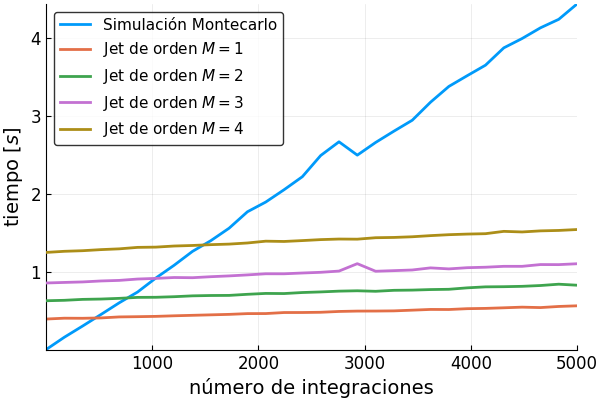
\includegraphics[width = \textwidth]{times_sp}
\end{subfigure}
%
\begin{subfigure}{0.49\textwidth}
	\centering
	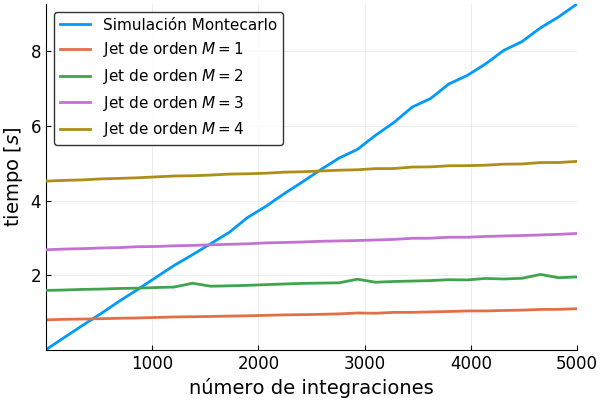
\includegraphics[width = \textwidth]{times_c3bp}
\end{subfigure}
\caption{Tiempo en segundos de cómputo en función del número de condiciones iniciales propagadas utilizando órdenes $M = \left\lbrace 1,2,3,4 \right\rbrace$ en dorado, violeta, verde y naranja, respectivamente. Las integraciones para ambos casos fueron realizadas con una tolerancia $\epsilon_{Taylor} = 10^{-18}$, orden de la expansión $N=20$ y $10$ pasos de integración que, en el caso del péndulo, corresponden a un periodo. \textit{Izquierda}: péndulo simple con condición inicial $\xo = \left(\pi/2, 0 \right)^T$. \textit{Derecha}: PC3C con condición inicial $\xo = \left(L_{4_x}, L_{4_y} + 0.01, 0, 0 \right)^T$ y $\mu = 0.012$, el parámetro Tierra-Luna.}
\label{fig:times}
\end{figure}

Se muestra en la figura \ref{fig:times} la integración de hasta $5000$ condiciones iniciales cercanas para el péndulo y el PC3C. En ambos casos se tiene un comportamiento parecido donde, para pocas integraciones, el método de Montecarlo es más rápido que el TJ. Esto se debe a la lentitud algebráica de los polinomios operados. Sin embargo, el tiempo que demora el TJ durante toda la gráfica es casi constante para todos los órdenes. Éste no es perfectamente constante dado que la evaluación de los polinomios sí requiere tiempo, aunque es mucho menor al de hacer una integración más. Es por esto que la pendiente que describe el aumento en el tiempo de cómputo es casi constante para el transporte de jets. En el caso de Montecarlo, se tiene aproximadamente una recta de pendiente positiva, lo cual es de esperarse ya que en la vecindad cada integración demora aproximadamente lo mismo. 

%FIGURE!
\begin{figure}[h!]
\centering
\begin{subfigure}{0.49\textwidth}
	\centering
	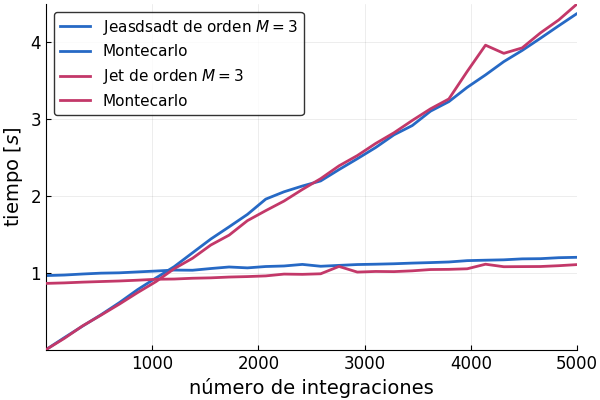
\includegraphics[width = \textwidth]{times_sp_diffx0}
\end{subfigure}
%
\begin{subfigure}{0.49\textwidth}
	\centering
	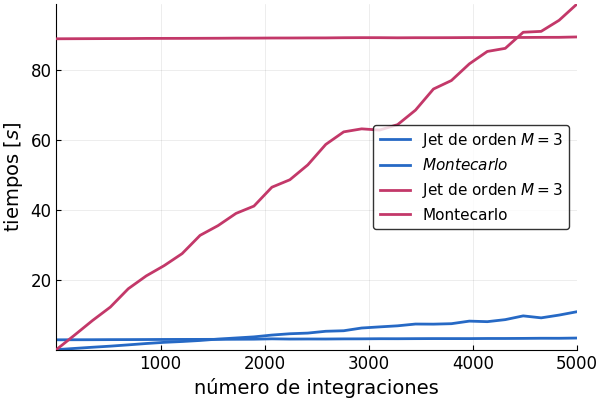
\includegraphics[width = \textwidth]{times_c3bp_diffx0}
\end{subfigure}
\caption{Tiempo en segundos de cómputo en función del número de integraciones utilizando diferentes condiciones iniciales. Ambos casos fueron realizados con una tolerancia $\epsilon_{Taylor} = 10^{-18}$, orden de la expansión $N=20$, orden del jet $M=3$ y $10$ pasos de integración que, en el caso del péndulo, corresponden a un periodo. \textit{Izquierda}: péndulo simple con condiciones inicial $\xo = \left(\pi/2, 0 \right)^T$ (azul) y $\xo = \left(15\pi/16, 0 \right)^T$ (magenta). \textit{Derecha}: PC3C con condiciones iniciales $\xo = \left(L_{4_x}, L_{4_y} + 0.01, 0, 0 \right)^T$ (azul) $\xo = \left(L_{1}, 0 + 0.01, 0, 0 \right)^T$ (magenta), con $\mu = 0.012$.}
\label{fig:times_diffx0}
\end{figure}

No todas las condiciones iniciales en el espacio fase tardan el mismo tiempo en integrarse para el mismo intervalo. Por esto, se presenta la figura \ref{fig:times_diffx0}, donde se observa la dependencia de cómputo en función de la condición inicial seleccionada. El comportamiento del TJ sigue siendo casi constante aunque escala de manera considerable para las dos condiciones evaluadas. En el PC3C se hace mucho más evidente donde, para $\xo = (L_{4_x}, L_{4_x} + 0.01, 0, 0)^T$, el tiempo promedio del transporte ya evaluado es de $89.1$ segundos, mientras que para $\xo = (L_1, 0.01, 0, 0)^T$ es de $3.05$ segundos.

Finalmente, para concluir el apéndice se presentan resultados de tiempo de cómputo para algunas operaciones elementales usando el álgebra polinomial. La tabla \ref{table:times_algpoli_1} presenta la velocidad de cómputo en escala logarítmica para polinomios de dos variables pero con orden de jet variable desde $1$ hasta $32$. Como referencia, la primera fila representa el tiempo que tarda hacer la misma operación elemental con un número de punto flotante arbitrario. 

%TABLA!
\begin{table}[h!]
\centering
\begin{tabular}{c|cccc}
\toprule
     & \textbf{$\sin$} & \textbf{$\cos$} & \textbf{$\exp$} & \textbf{$\log$} \\ \cmidrule(l){1-5} 
$M=0$  & $-8.02$ & $-8.02$ & $-8.12$ & $-8.0 $ \\
$M=1$  & $-6.06$ & $-6.06$ & $-6.38$ & $-6.34$ \\
$M=2$  & $-5.87$ & $-5.88$ & $-6.18$ & $-6.13$ \\
$M=4$  & $-5.59$ & $-5.59$ & $-5.91$ & $-5.85$ \\
$M=8$  & $-5.2 $ & $-5.2 $ & $-5.5 $ & $-5.48$ \\
$M=16$ & $-4.73$ & $-4.73$ & $-5.05$ & $-5.02$ \\
$M=32$ & $-4.14$ & $-4.14$ & $-4.45$ & $-4.44$ \\ \bottomrule 
\end{tabular}
\caption{Logaritmo base $10$ del tiempo que demora hacer cada operación elemental para polinomios $P(\mathbf{x}) \in \pkk{M}{2}$, es decir, polinomios en dos variables de orden $M$. $M=0$ representa la operación aritmética con un número flotante arbitrario.}
\label{table:times_algpoli_1}
\end{table}

La tabla \ref{table:times_algpoli_2}, en cambio, mantiene constante el orden del jet a $M=3$ pero cambia el numero de variables para cada operación. En todos los casos se evaluó la operación elemental en la primera variable independiente del polinomio, pero tomando en cuenta que $P(\mathbf{x}) \in \pkk{3}{n}$, con $n \in \left\lbrace 1,2,3,4,5 \right\rbrace$. 

%TABLA!
\begin{table}[h!]
\centering
\begin{tabular}{c|cccc}
\toprule
     & \textbf{$\sin$} & \textbf{$\cos$} & \textbf{$\exp$} & \textbf{$\log$} \\ \cmidrule(l){1-5} 
 $\#_{vars} = 0$ & $-8.02$ & $-8.02$ & $-8.12$ & $-8.00$ \\
 $\#_{vars} = 1$ & $-5.68$ & $-5.68$ & $-5.98$ & $-5.92$ \\
 $\#_{vars} = 2$ & $-5.60$ & $-5.59$ & $-5.90$ & $-5.84$ \\
 $\#_{vars} = 3$ & $-5.56$ & $-5.56$ & $-5.87$ & $-5.82$ \\
 $\#_{vars} = 4$ & $-5.53$ & $-5.53$ & $-5.84$ & $-5.80$ \\
 $\#_{vars} = 5$ & $-5.47$ & $-5.47$ & $-5.78$ & $-5.74$ \\ \bottomrule 
\end{tabular}
\caption{Logaritmo base $10$ del tiempo que demora hacer cada operación elemental para polinomios $P(\mathbf{x}) \in \pkk{3}{n}$, es decir, polinomios en $n$ variables de orden $M = 3$. $\#_{vars}=0$ representa la operación aritmética con un número flotante arbitrario.}
\label{table:times_algpoli_2}
\end{table}

